% Insert with \input from the ACL main file; do not compile this file alone.
\begingroup
\graphicspath{{figures/data_extraction_example/acl/}}
\definecolor{ink}{gray}{0.05}
\definecolor{muted}{gray}{0.35}
\definecolor{line}{gray}{0.55}
% Exact three-method palette from notebooks/eval/eval_summary.ipynb:
% Direct = blue, Workflow = yellow, MAS = magenta.
\definecolor{plotblue}{HTML}{007DCC}
\definecolor{plotyellow}{HTML}{FFB900}
\definecolor{plotmagenta}{HTML}{D10056}
\colorlet{bluewash}{plotblue!9}
\colorlet{yellowwash}{plotyellow!15}
\colorlet{magentawash}{plotmagenta!9}

\newcommand{\extractionscreenshotmark}[5]{%
  \fill[#1,opacity=.10] (#2,#3) rectangle (#4,#5);%
  \draw[#1,line width=1.1pt] (#2,#3) rectangle (#4,#5);%
}
\newcommand{\extractionpaperpage}[3]{%
  \node[anchor=south west,inner sep=0] at (#1,#2)
    {\includegraphics[page=#3,width=3.12cm,height=4.16cm]{paper.pdf}};%
  \draw[draw=line,line width=.5pt] (#1,#2) rectangle ++(3.12,4.16);%
}
\newcommand{\extractionfield}[5]{%
  \fill[#5] (#1,2.64) rectangle ({#1+#2},3.33);%
  \node[font=\rmfamily\fontsize{7}{8}\selectfont,align=center,text=muted] at ({#1+#2/2},2.985) {#3};%
  \node[font=\rmfamily\bfseries\fontsize{8.5}{9}\selectfont,align=center,text=ink] at ({#1+#2/2},2.285) {#4};%
}
\tikzset{tableline/.style={draw=line,line width=.5pt}}
\begin{tikzpicture}[x=1cm,y=1cm,>=Latex]
  \path[use as bounding box] (0,.72) rectangle (26.2,10.96);
  \fill[white] (0,.72) rectangle (26.2,10.96);

  % Paper stack. The front is the original first page; pages 27 and 29 sit behind it.
  \begin{scope}
    \extractionpaperpage{1.22}{6.00}{5}
    \extractionpaperpage{0.92}{6.26}{3}
    \extractionpaperpage{0.62}{6.52}{1}
  \end{scope}
  \node[anchor=west,font=\rmfamily\bfseries\fontsize{9}{10}\selectfont,text=ink] at (.62,5.73) {Source paper};
  \draw[-{Latex[length=2.5mm]},line width=1.1pt,draw=muted] (4.05,8.35) -- (4.53,8.35);

  % Three screenshot cards, retaining the user's left-to-right evidence order.
  \foreach \xa/\xb in {4.66/10.54,10.67/16.55,16.68/25.60}{
    \draw[fill=white,draw=line,line width=.5pt]
      (\xa,5.79) rectangle (\xb,10.78);
  }
  \node[anchor=north west,inner sep=0] at (4.80,10.38)
    {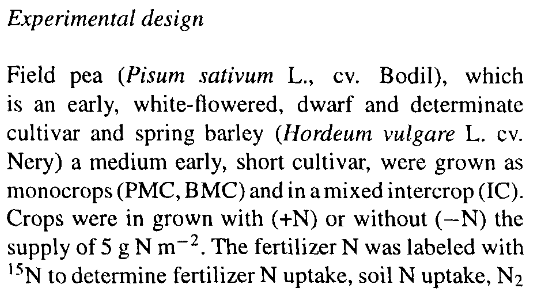
\includegraphics[width=5.60cm]{design.png}};
  \node[anchor=north west,inner sep=0] at (10.81,10.38)
    {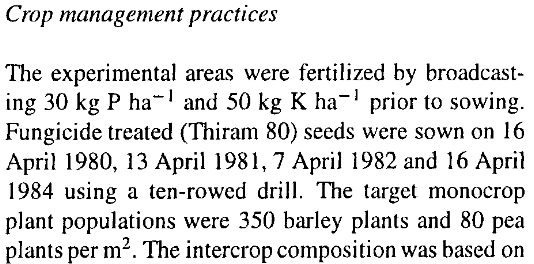
\includegraphics[width=5.60cm]{management.png}};
  \node[anchor=north west,inner sep=0] at (16.82,10.38)
    {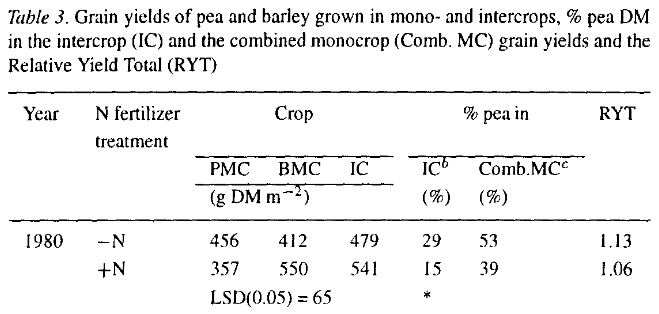
\includegraphics[width=8.60cm]{results.png}};

  % Pixel-aligned highlights. Negative y in these scopes means pixels run down the image.
  \begin{scope}[shift={(4.80,10.38)},x=.0104869cm,y=-.0104869cm]
    \extractionscreenshotmark{plotblue}{3}{62}{108}{91}
    \extractionscreenshotmark{plotblue}{143}{122}{327}{149}
    \extractionscreenshotmark{plotblue}{429}{207}{496}{234}
  \end{scope}
  \begin{scope}[shift={(10.81,10.38)},x=.0104869cm,y=-.0104869cm]
    \extractionscreenshotmark{plotyellow}{493}{117}{530}{146}
    \extractionscreenshotmark{plotyellow}{4}{149}{112}{177}
  \end{scope}
  \begin{scope}[shift={(16.82,10.38)},x=.0130501cm,y=-.0130501cm]
    \extractionscreenshotmark{plotmagenta}{18}{225}{68}{254}
    \extractionscreenshotmark{plotmagenta}{91}{225}{137}{254}
    \extractionscreenshotmark{plotmagenta}{203}{225}{244}{254}
    \extractionscreenshotmark{plotmagenta}{273}{225}{313}{254}
    \extractionscreenshotmark{plotmagenta}{344}{225}{386}{254}
    \extractionscreenshotmark{plotmagenta}{419}{225}{451}{254}
    \extractionscreenshotmark{plotmagenta}{592}{225}{638}{254}
  \end{scope}

  \node[anchor=west,font=\rmfamily\bfseries\fontsize{9}{10}\selectfont,text=ink] at (4.83,6.23) {1\quad Crops and treatment};
  \node[anchor=west,font=\rmfamily\fontsize{8}{9}\selectfont,text=muted] at (4.83,5.93) {p.~26 / PDF page 2};
  \node[anchor=west,font=\rmfamily\bfseries\fontsize{9}{10}\selectfont,text=ink] at (10.84,6.23) {2\quad Year};
  \node[anchor=west,font=\rmfamily\fontsize{8}{9}\selectfont,text=muted] at (10.84,5.93) {p.~27 / PDF page 3};
  \node[anchor=west,font=\rmfamily\bfseries\fontsize{9}{10}\selectfont,text=ink] at (16.85,6.23) {3\quad Yield results};
  \node[anchor=west,font=\rmfamily\fontsize{8}{9}\selectfont,text=muted] at (16.85,5.93) {p.~29 / PDF page 5, Table 3};

  % Map each evidence card to one segment of the same ground-truth record.
  \draw[-{Latex[length=2mm]},draw=plotblue,line width=.9pt] (7.60,5.75) -- (7.60,4.95);
  \draw[-{Latex[length=2mm]},draw=plotyellow,line width=.9pt] (13.61,5.75) -- (13.61,4.95);
  \draw[-{Latex[length=2mm]},draw=plotmagenta,line width=.9pt] (21.12,5.75) -- (21.12,4.95);

  \node[anchor=west,align=left,font=\rmfamily\bfseries\fontsize{10}{11}\selectfont,text=ink] at (.62,2.60)
    {Ground truth:\\one curated data row};
  \node[anchor=east,font=\rmfamily\fontsize{8}{9}\selectfont,text=muted] at (25.54,4.61)
    {selected columns from Study 1 / T-1};

  \node[anchor=west,font=\rmfamily\bfseries\fontsize{8}{9}\selectfont,text=ink] at (4.74,3.83) {Experimental context};
  \node[anchor=west,font=\rmfamily\bfseries\fontsize{8}{9}\selectfont,text=ink] at (10.75,3.83) {Record identity};
  \node[anchor=west,font=\rmfamily\bfseries\fontsize{8}{9}\selectfont,text=ink] at (16.75,3.83) {Yield and derived ratio};

  \extractionfield{4.74}{1.44}{Crop 1}{Barley}{bluewash}
  \extractionfield{6.18}{1.44}{Crop 2}{Pea}{bluewash}
  \extractionfield{7.62}{1.44}{N IC1}{0}{bluewash}
  \extractionfield{9.06}{1.44}{N IC2}{0}{bluewash}

  \extractionfield{10.75}{1.92}{Study\#}{1}{yellowwash}
  \extractionfield{12.67}{1.92}{Rec\#}{T-1}{yellowwash}
  \extractionfield{14.59}{1.92}{Year}{1980}{yellowwash}

  \extractionfield{16.75}{1.76}{Yield SC1}{412}{magentawash}
  \extractionfield{18.51}{1.76}{Yield SC2}{456}{magentawash}
  \extractionfield{20.27}{1.76}{Yield IC1$^{*}$}{340.09}{magentawash}
  \extractionfield{22.03}{1.76}{Yield IC2$^{*}$}{138.91}{magentawash}
  \extractionfield{23.79}{1.95}{LER$^{*}$}{\fontsize{8}{8}\selectfont 1.130088358}{magentawash}

  % Draw each border once, after the cell fills, for uniform weight and color.
  \foreach \left/\right in {4.74/10.50,10.75/16.51,16.75/25.74}{
    \draw[tableline] (\left,1.93) rectangle (\right,3.33);
    \draw[tableline] (\left,2.64) -- (\right,2.64);
  }
  \foreach \sep in {6.18,7.62,9.06,12.67,14.59,18.51,20.27,22.03,23.79}{
    \draw[tableline] (\sep,1.93) -- (\sep,3.33);
  }

  \node[anchor=west,font=\rmfamily\fontsize{8}{9}\selectfont,text=muted] at (4.74,1.43)
    {SC = sole crop; IC = intercrop. Yields are g/m$^2$. Crop 1 is barley and crop 2 is pea.};
  \node[anchor=west,font=\rmfamily\fontsize{8}{9}\selectfont,text=muted] at (4.74,1.06)
    {$^{*}$Calculated by the ground-truth curator: pea $=479\times0.29=138.91$; barley $=479\times0.71=340.09$; LER $=340.09/412+138.91/456$.};
\end{tikzpicture}
\endgroup
